\documentclass[11pt, oneside]{article}   	% use "amsart" instead of "article" for AMSLaTeX format
\usepackage[margin=1in]{geometry}                		% See geometry.pdf to learn the layout options. There are lots.
\geometry{letterpaper}                   		% ... or a4paper or a5paper or ... 
%\geometry{landscape}                		% Activate for rotated page geometry
%\usepackage[parfill]{parskip}    		% Activate to begin paragraphs with an empty line rather than an indent
\usepackage{graphicx}				% Use pdf, png, jpg, or eps§ with pdflatex; use eps in DVI mode
								% TeX will automatically convert eps --> pdf in pdflatex		
\usepackage{amssymb}
\usepackage{courier}
%usepackage{undertilde}
\usepackage[numbered,framed]{matlab-prettifier}
\usepackage{framed}

\usepackage[T1]{fontenc}
\usepackage{mathtools}  % loads »amsmath«
\usepackage{physics}
\usepackage{listings}

\lstset{
  language=C,                % choose the language of the code
  numbers=left,                   % where to put the line-numbers
  stepnumber=1,                   % the step between two line-numbers.        
  numbersep=5pt,                  % how far the line-numbers are from the code
  backgroundcolor=\color{white},  % choose the background color. You must add \usepackage{color}
  showspaces=false,               % show spaces adding particular underscores
  showstringspaces=false,         % underline spaces within strings
  showtabs=false,                 % show tabs within strings adding particular underscores
  tabsize=2,                      % sets default tabsize to 2 spaces
  captionpos=b,                   % sets the caption-position to bottom
  breaklines=true,                % sets automatic line breaking
  breakatwhitespace=true,         % sets if automatic breaks should only happen at whitespace
  title=\lstname,                 % show the filename of files included with \lstinputlisting;
}

\setlength{\parskip}{0.5em}

%SetFonts
\newcommand\Rey{\mbox{\textit{Re}}}

\title{\vspace{-6ex}\large PHYS 516: Methods of Computational Physics \\ [1ex]
 ASSIGNMENT 7- RANDOM WALKS\vspace{-3ex}}
\author{Anup V Kanale}
\date{\vspace{-3ex}\today}							% Activate to display a given date or no date

\begin{document}
\vspace{-6ex}\maketitle

\section{\vspace{-1ex}Stock price simulation}
This section illustrates the application of MC simulation to a stochastic problem-- Stock price in this case specifically. \vspace{-2ex}

\subsection{\vspace{-2ex} MC simulations of stock price based on Black-Scholes Model}	
A program was written in C to perform Monte Carlo (MC) simulations of a stock price, $S$, as a function of time, $t$, assuming that $S$ follows a discrete stochastic equation
	\begin{equation}
		dS = \mu S dt + \sigma \varepsilon S \sqrt{dt}
	\end{equation}
where $dt$ is the time discretization unit and $\varepsilon$ is a random variable following the normal distribution with unit variance. The code is attached in the appendix at the end of the report.\vspace{-2ex}

\subsection{\vspace{-2ex} Temporal variation of stock price}
A simulation was run to see the variation of stock price over time. There are 100 random walker (or investors), the starting stock price was chosen as \$20.0 and a 14 \% per annum ($\mu = 0.14$) expected return with a standard deviation of 20\% per annum ($\sigma = 0.20$) was used. Let dt = 0.00274 year (~1 day). The MC simulation was run for 1 year (365 steps).

The variation of the stock price is as shown in figure \ref{stock}. The matlab script for plotting is included in the Appendix.
	\begin{figure}[!htbp] \label{stock}
	\centering
	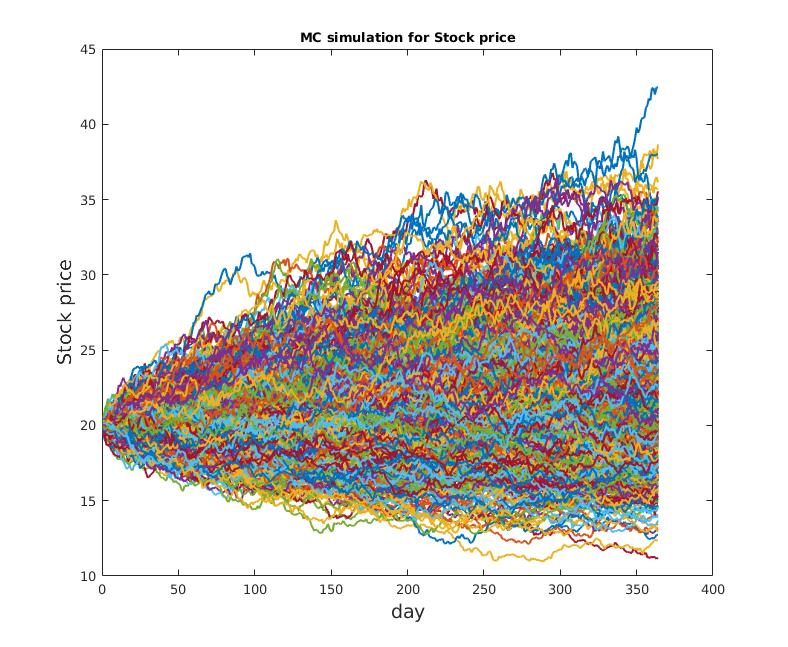
\includegraphics[scale=0.35]{stockPricePlot.jpg}
	\caption{Variation of stock price over the year for 1000 investors}
	\end{figure}

\subsection{\vspace{-2ex} Histogram of stock price}
The MC simulations were repeated 1,000 times with the same parameters, but with different random number seeds. The histogram below in figure \ref{hist} shows the number of random walkers (or investors) at each given price of stock at the end of the year.
	\begin{figure}[!htbp] \label{hist}
	\centering
	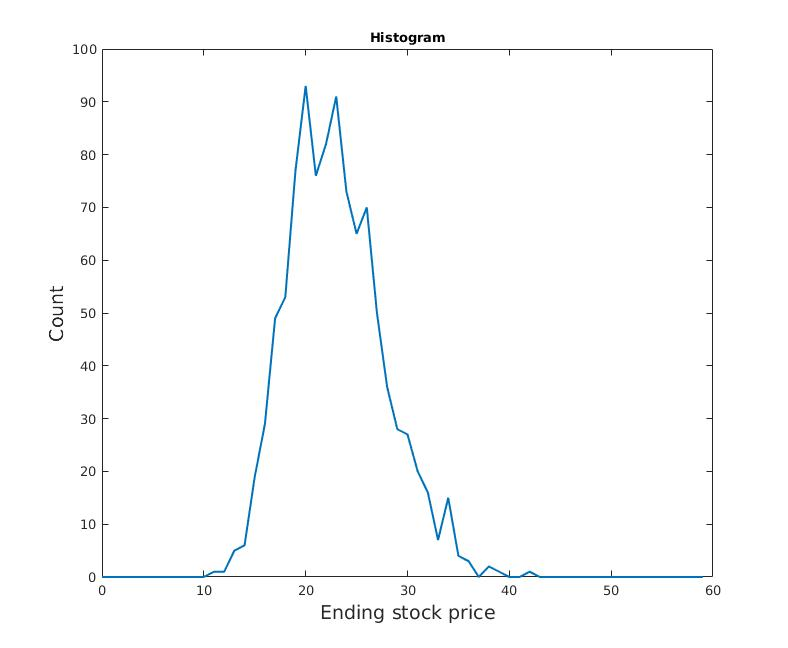
\includegraphics[scale=0.35]{stockHistogram.jpg}
	\caption{Histogram at the end of the year for 1000 investors}
	\end{figure}

As the number of investors is increased, the histogram gradually becomes a smooth Gaussian, as is seen from figure \ref{increase}
	\begin{figure}[!htbp] \label{increase}
	\centering
	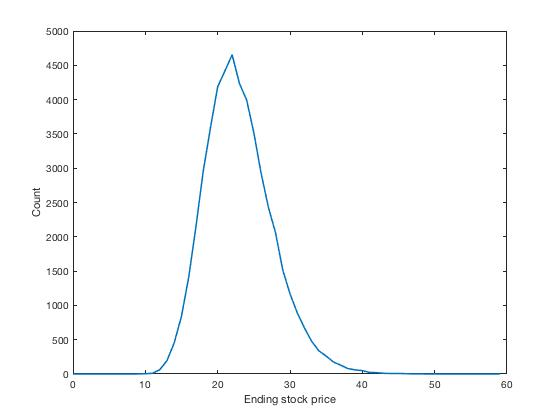
\includegraphics[scale=0.5]{stockHistogram50000.jpg}
	\caption{Histogram at the end of the year for 50000 investors}
	\end{figure}

\pagebreak
\section{\vspace{-1ex}Quantum Monte Carlo simulation}
This section illustrates the quantum Monte Carlo technique. The difference from Part I is that while simulating the electron wave function, in addition to the diffusion term, a birth/death term exists in the Imaginary-time Schrodinger Equation. \vspace{-2ex}

\subsection{\vspace{-2ex} Quantum Monte Carlo Simulation of 1D Diffusion problem}
A program was written to simulate diffusion using quantum Monte Carlo simulation of a 1D electron wave function, in a harmonic potential given by $V(x) = x^2/2$ (in the atomic unit). The program is attached in appendix A. The energy as a function of MC steps is shown in figure \ref{energy}
	\begin{figure}[!htbp] \label{energy}
	\centering
	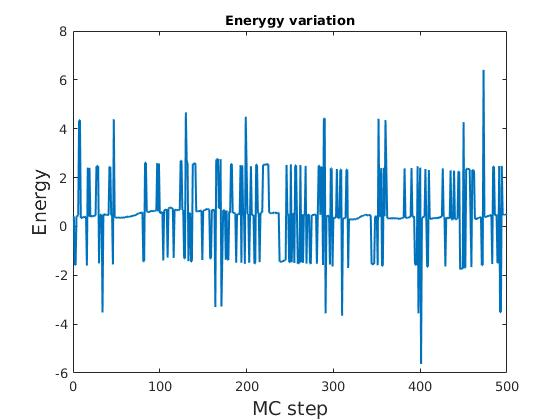
\includegraphics[scale=0.45]{energyVariation.jpg}
	\caption{Energy variation with MC step}
	\end{figure} \vspace{-2ex}
	
\subsection{\vspace{-2ex} Histogram}
The histogram of random walkers is shown in figure \ref{qmc}
	\begin{figure}[!htbp] \label{qmc}
	\centering
	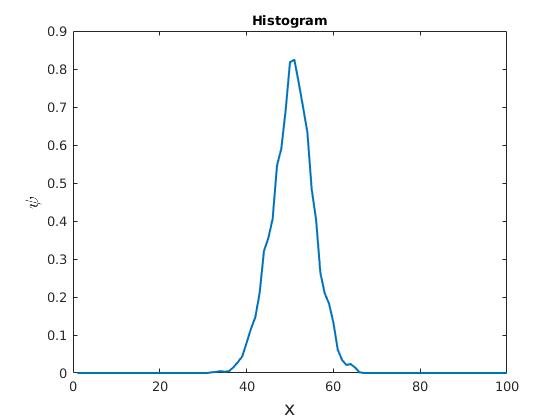
\includegraphics[scale=0.45]{qmcHistogram.jpg}
	\caption{Histogram of random walkers}
	\end{figure}

\pagebreak
\appendix
\section{C Programs for simulation}
\lstinputlisting[language=C, frame=single]{stockPriceMC.c}
\lstinputlisting[language=C, frame=single]{quantumMC.c}
\section{Matlab scripts for plotting}
\lstinputlisting[style=Matlab-editor]{stockPricePlots.m}
\lstinputlisting[style=Matlab-editor]{qmcPlots.m}

\end{document}